\usetikzlibrary{fit,matrix}
\usetikzlibrary{arrows.meta,calc,shapes}
\providecommand{\computer}{%
    
\includegraphics[width=1cm]{../common/Noun_project_216.pdf}
}
\providecommand{\switch}{%
    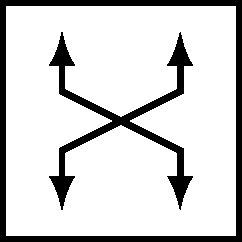
\includegraphics[width=0.9cm]{../common/fig-switch.pdf}
}
\providecommand{\router}{%
    
\includegraphics[width=0.9cm]{../common/fig-router.pdf}
}
\begin{frame}{switch v router: tables}
\begin{tikzpicture}
\matrix[tight matrix,
    nodes={minimum height=.6cm},
    column 1/.style={nodes={text width=5cm,font=\small\tt}},
    column 2/.style={nodes={text width=1cm,font=\small\tt}},
    row 1/.style={nodes={font=\small}},
    label={north:switch (`bridge') table},
] (bridge table) {
MAC address \& port \\
00:11:22:33:44:55 \& 1 \\
00:33:00:01:02:aa \& 2 \\
00:44:00:01:02:bb \& 3 \\
\ldots \& \ldots \\
\normalfont default \& (all) \\
};
\matrix[tight matrix,
    nodes={minimum height=.6cm},
    column 1/.style={nodes={text width=4.5cm,font=\small\tt}},
    column 2/.style={nodes={text width=2cm,font=\small\tt,alt=<4>{fill=red!10}}},
    column 3/.style={nodes={text width=1cm,font=\small\tt,alt=<3>{fill=red!10}}},
    row 1/.style={nodes={font=\small}},
    label={north:routing table},
    anchor=north west
] (route table) at ([xshift=.5cm]bridge table.north east){
IP addresses \& gateway \& iface \\
2001:0db8:40::/48 \& --- \& int \\
3fff:1000:19::/48 \& --- \& ext \\
\ldots \& \ldots \& \ldots \\
\normalfont default \& fe80::17 \& ext \\
};
\begin{visibleenv}<2>
\node[
    draw=red,ultra thick,fit=(bridge table),
] (bridge table around) {};
\node[align=left,anchor=north west] at (bridge table around.south west) {
    one logical device with multiple ports \\
    not in table: always broadcast
};
\end{visibleenv}
\begin{visibleenv}<3->
\node[
    draw=red,ultra thick,fit=(route table),
] (route table around) {};
\end{visibleenv}
\begin{visibleenv}<3>
\node[align=left,anchor=north] at (route table around.south) {
    `interface' = which network \\
    ~ \\
    one interface might have multiple ports \\
    that are `bridged' together \\
};
\end{visibleenv}
\begin{visibleenv}<4>
\node[align=left,anchor=north] at (route table around.south) {
    gateway = who to send to next \\
    no gateway = `direct' to destination \\
    ~ \\
    need to have specific destination \\
    to send to on interface
};
\end{visibleenv}
\end{tikzpicture}
\end{frame}

\begin{frame}{aside: trivial tables}
\begin{itemize}
\item let's say we're connected to ONE interface with ONE port
\item<2-> tables are really trivial:
\end{itemize}
\begin{visibleenv}<2->
\begin{tikzpicture}
\matrix[tight matrix,
    nodes={minimum height=.6cm},
    column 1/.style={nodes={text width=5cm,font=\small\tt}},
    column 2/.style={nodes={text width=1cm,font=\small\tt}},
    row 1/.style={nodes={font=\small}},
    label={north:switch (`bridge') table},
] (bridge table) {
MAC address \& port \\
default \& the port \\
};
\matrix[tight matrix,
    nodes={minimum height=.6cm},
    column 1/.style={nodes={text width=4.5cm,font=\small\tt}},
    column 2/.style={nodes={text width=2cm,font=\small\tt,alt=<4>{fill=red!10}}},
    column 3/.style={nodes={text width=4cm,font=\fontsize{9}{10}\tt,alt=<3>{fill=red!10}}},
    row 1/.style={nodes={font=\small}},
    label={north:routing table (IPv6)},
    anchor=north west
] (route table) at ([xshift=.5cm]bridge table.north east){
IP addresses \& gateway \& iface \\
2001:0db8:40::/48 \& --- \& the interface \\
\normalfont default \& fe80::17 \& the interface \\
};
\matrix[tight matrix,
    nodes={minimum height=.6cm},
    column 1/.style={nodes={text width=4.5cm,font=\small\tt}},
    column 2/.style={nodes={text width=2cm,font=\small\tt,alt=<4>{fill=red!10}}},
    column 3/.style={nodes={text width=4cm,font=\fontsize{9}{10}\tt,alt=<3>{fill=red!10}}},
    row 1/.style={nodes={font=\small}},
    label={north:routing table (IPv4)},
    anchor=north west
] (route table) at ([xshift=.5cm]bridge table.north east){
IP addresses \& gateway \& iface \\
192.0.2.0/24 \& --- \& the interface \\
\normalfont default \& 192.0.2.1 \& the interface \\
};
\end{tikzpicture}
\end{visibleenv}
\end{frame}
